\chapter{Hasil dan Analisis}

\section{Hasil}

Gambar \ref{fig:node119} sampai dengan \ref{fig:node720} menunjukkan perbandingan suhu \textit{node-node} satelit
hasil prediksi model termal dengan data telemetri aktual LAPAN-A3 untuk periode observasi 19 sampai dengan 20 Mei 2018.

\begin{figure}[H]
\setlength\belowcaptionskip{-0.7\baselineskip}
\begin{center}
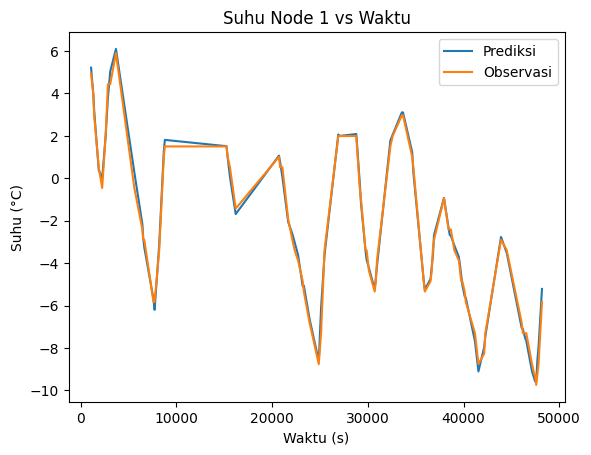
\includegraphics[width=0.6\textwidth]{fig/node1_temp_2018-05-19.png}
	\caption{Grafik Suhu \textit{Node} 1 vs Waktu 19 Mei 2018}
\label{fig:node119}
\end{center}
\end{figure}

\begin{figure}[H]
\setlength\belowcaptionskip{-0.7\baselineskip}
\begin{center}
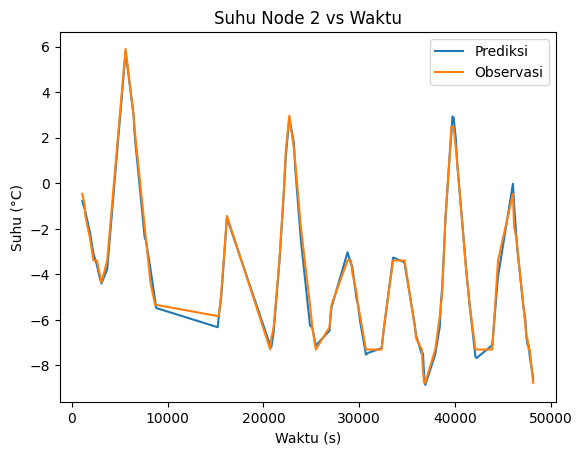
\includegraphics[width=0.6\textwidth]{fig/node2_temp_2018-05-19.png}
	\caption{Grafik Suhu \textit{Node} 2 vs Waktu 19 Mei 2018}
\label{fig:node219}
\end{center}
\end{figure}

\begin{figure}[H]
\setlength\belowcaptionskip{-0.7\baselineskip}
\begin{center}
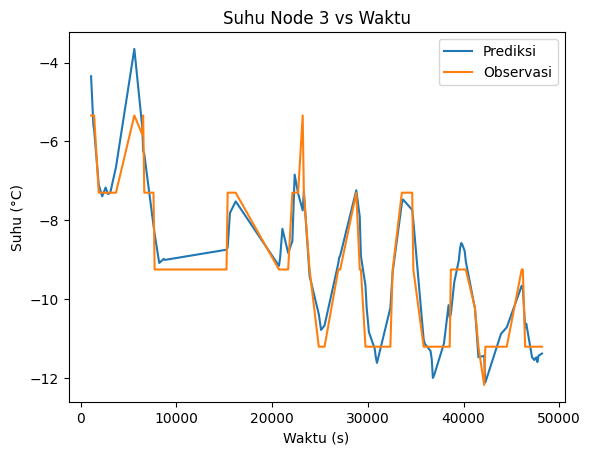
\includegraphics[width=0.6\textwidth]{fig/node3_temp_2018-05-19.png}
	\caption{Grafik Suhu \textit{Node} 3 vs Waktu 19 Mei 2018}
\label{fig:node319}
\end{center}
\end{figure}

\begin{figure}[H]
\setlength\belowcaptionskip{-0.7\baselineskip}
\begin{center}
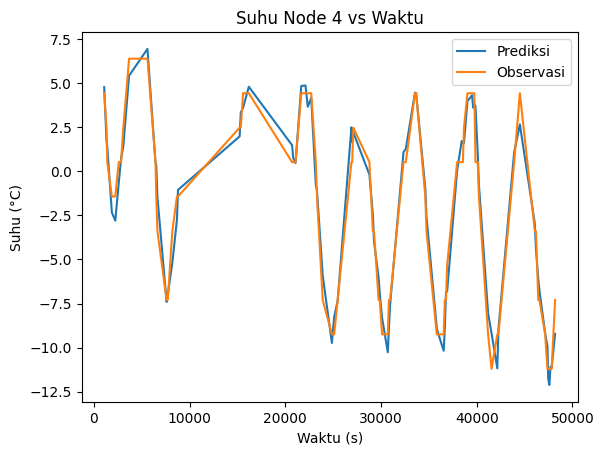
\includegraphics[width=0.6\textwidth]{fig/node4_temp_2018-05-19.png}
	\caption{Grafik Suhu \textit{Node} 4 vs Waktu 19 Mei 2018}
\label{fig:node419}
\end{center}
\end{figure}

\begin{figure}[H]
\setlength\belowcaptionskip{-0.7\baselineskip}
\begin{center}
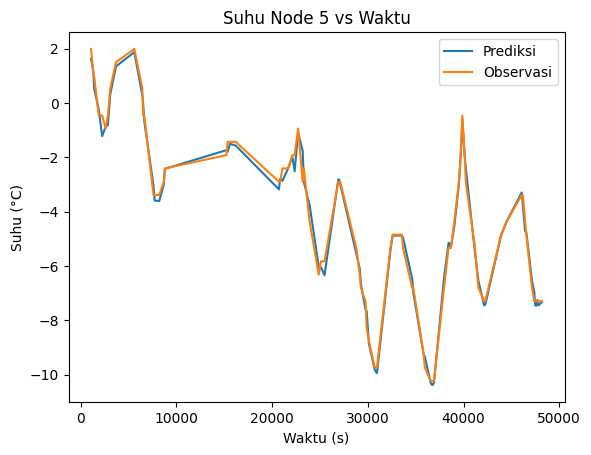
\includegraphics[width=0.6\textwidth]{fig/node5_temp_2018-05-19.png}
	\caption{Grafik Suhu \textit{Node} 5 vs Waktu 19 Mei 2018}
\label{fig:node519}
\end{center}
\end{figure}

\begin{figure}[H]
\setlength\belowcaptionskip{-0.7\baselineskip}
\begin{center}
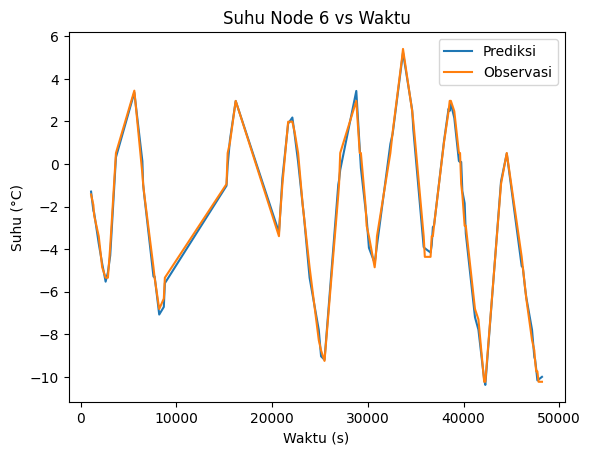
\includegraphics[width=0.6\textwidth]{fig/node6_temp_2018-05-19.png}
	\caption{Grafik Suhu \textit{Node} 6 vs Waktu 19 Mei 2018}
\label{fig:node619}
\end{center}
\end{figure}

\begin{figure}[H]
\setlength\belowcaptionskip{-0.7\baselineskip}
\begin{center}
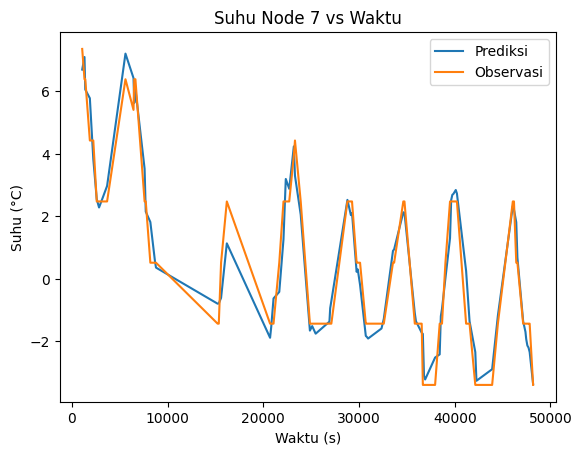
\includegraphics[width=0.6\textwidth]{fig/node7_temp_2018-05-19.png}
\caption{Grafik Suhu \textit{Node} 7 vs Waktu 19 Mei 2018}
\label{fig:node719}
\end{center}
\end{figure}

\begin{figure}[H]
\setlength\belowcaptionskip{-0.7\baselineskip}
\begin{center}
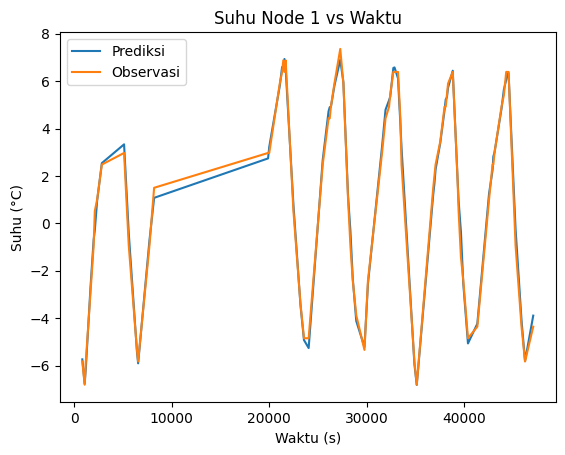
\includegraphics[width=0.6\textwidth]{fig/node1_temp_2018-05-20.png}
\caption{Grafik Suhu \textit{Node} 1 vs Waktu 20 Mei 2018}
\label{fig:node120}
\end{center}
\end{figure}

\begin{figure}[H]
\setlength\belowcaptionskip{-0.7\baselineskip}
\begin{center}
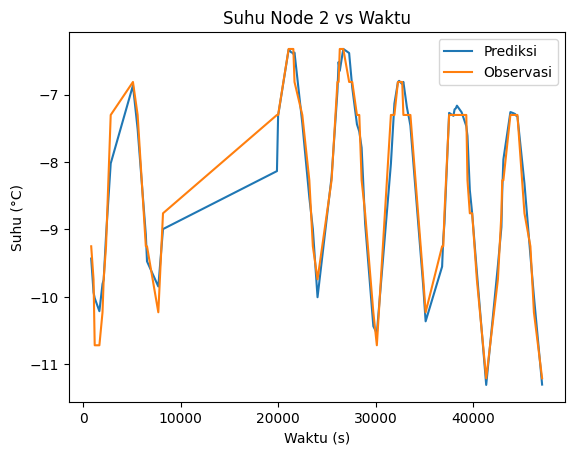
\includegraphics[width=0.6\textwidth]{fig/node2_temp_2018-05-20.png}
\caption{Grafik Suhu \textit{Node} 2 vs Waktu 20 Mei 2018}
\label{fig:node220}
\end{center}
\end{figure}

\begin{figure}[H]
\setlength\belowcaptionskip{-0.7\baselineskip}
\begin{center}
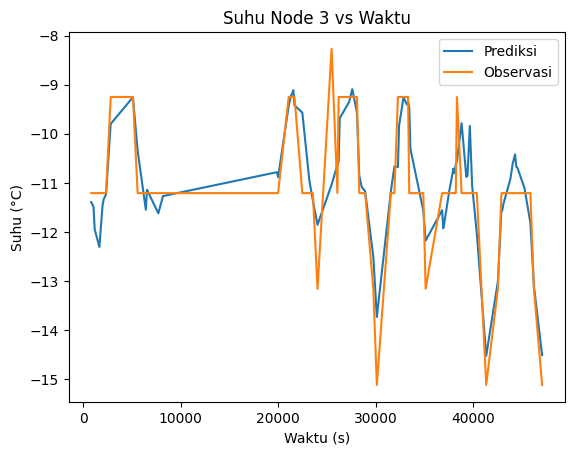
\includegraphics[width=0.6\textwidth]{fig/node3_temp_2018-05-20.png}
\caption{Grafik Suhu \textit{Node} 3 vs Waktu 20 Mei 2018}
\label{fig:node320}
\end{center}
\end{figure}

\begin{figure}[H]
\setlength\belowcaptionskip{-0.7\baselineskip}
\begin{center}
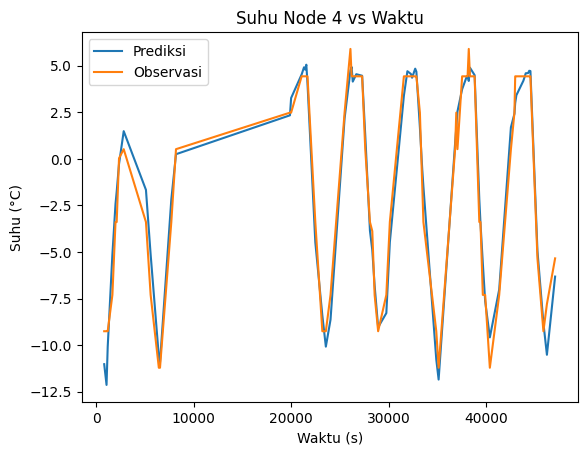
\includegraphics[width=0.6\textwidth]{fig/node4_temp_2018-05-20.png}
\caption{Grafik Suhu \textit{Node} 4 vs Waktu 20 Mei 2018}
\label{fig:node420}
\end{center}
\end{figure}

\begin{figure}[H]
\setlength\belowcaptionskip{-0.7\baselineskip}
\begin{center}
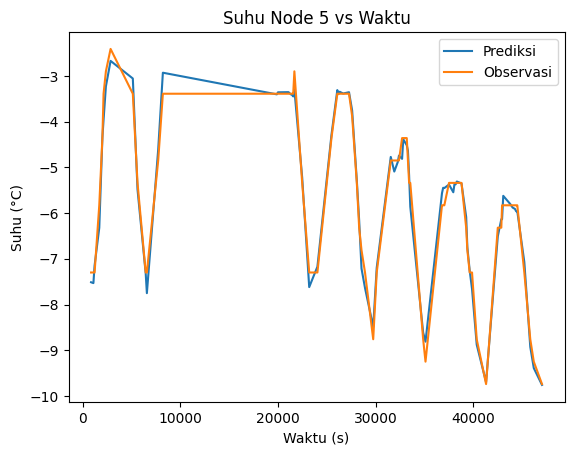
\includegraphics[width=0.6\textwidth]{fig/node5_temp_2018-05-20.png}
\caption{Grafik Suhu \textit{Node} 5 vs Waktu 20 Mei 2018}
\label{fig:node520}
\end{center}
\end{figure}

\begin{figure}[H]
\setlength\belowcaptionskip{-0.7\baselineskip}
\begin{center}
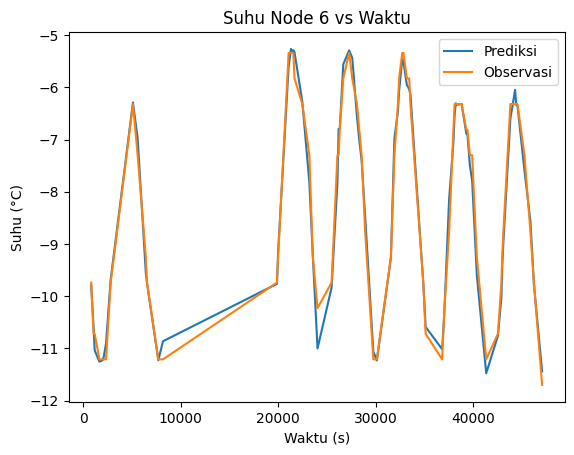
\includegraphics[width=0.6\textwidth]{fig/node6_temp_2018-05-20.png}
\caption{Grafik Suhu \textit{Node} 6 vs Waktu 20 Mei 2018}
\label{fig:node620}
\end{center}
\end{figure}

\begin{figure}[H]
\setlength\belowcaptionskip{-0.7\baselineskip}
\begin{center}
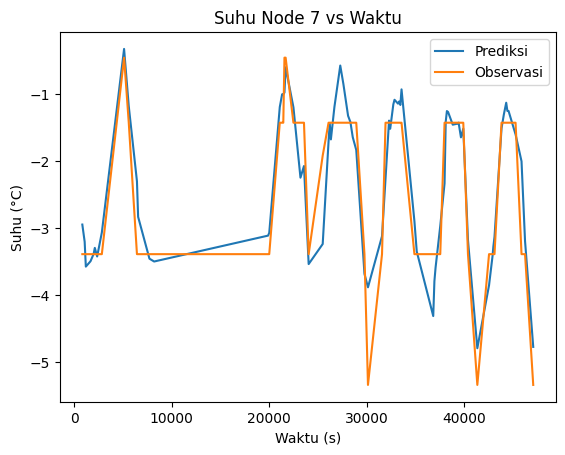
\includegraphics[width=0.6\textwidth]{fig/node7_temp_2018-05-20.png}
\caption{Grafik Suhu \textit{Node} 7 vs Waktu 20 Mei 2018}
\label{fig:node720}
\end{center}
\end{figure}

Dapat dilihat bahwa model termal LAPAN-A3 dapat memprediksi kebanyakan tren
perubahan suhu \texit{node-node} satelit selama periode observasi dengan akurasi yang
cukup dekat dengan suhu observasi. Meskipun prediksi model termal mengalami
\textit{overshoot} dan \textit{undershoot}, model termal secara umum dapat
memprediksi apakah suhu \texit{node-node} satelit akan naik, turun, atau tetap sama
pada setiap selang waktu.

Meski demikian, node 3 dan 7 menghasilkan prediksi suhu
dengan tren yang cukup kontras dengan data suhu observasi. Perbedaan tren
prediksi suhu untuk kedua node terlihat paling jelas pada Gambar \ref{fig:node320}
dan \ref{fig:node720} yang memuat plot suhu \textit{node} 3 dan 7 terhadap waktu untuk
periode observasi 20 Mei 2018. Dari kedua grafik tersebut, dapat dilihat bahwa
model termal memprediksi perubahan suhu \textit{node} meski data telemetri suhu node
konstan seperti yang terjadi pada rentang waktu 10000 sampai dengan 20000
sekon.

Agar dapat dinilai secara kuantitatif, performa model termal dalam memprediksi
tren perubahan suhu \texit{node-node} satelit dapat dilihat dari hasil perhitungan skor
R2 prediksi suhu \texit{node-node} satelit pada Gambar \ref{fig:r219} dan
\ref{fig:r220}. Model termal LAPAN-A3 dapat menjelaskan mayoritas varians suhu
\textit{node} sehingga menghasilkan skor R2 lebih dari 0.5 untuk semua \textit{node}. Lebih
lanjut, 6 dari 7 \textit{node} untuk periode 19 Mei 2018 dan 5 dari 7 \textit{node} untuk periode
20 Mei 2018 memiliki skor R2 lebih besar dari 0.9. Ini berarti lebih dari 90\%
varians dalam data suhu observasi dapat dijelaskan oleh prediksi model. Dapat
dilihat juga bahwa \textit{node} 3 memiliki skor R2 paling rendah dari ketujuh \textit{node} pada
kedua periode observasi dan disusul oleh \textit{node} 7.

\begin{figure}[H]
\setlength\belowcaptionskip{-0.7\baselineskip}
\begin{center}
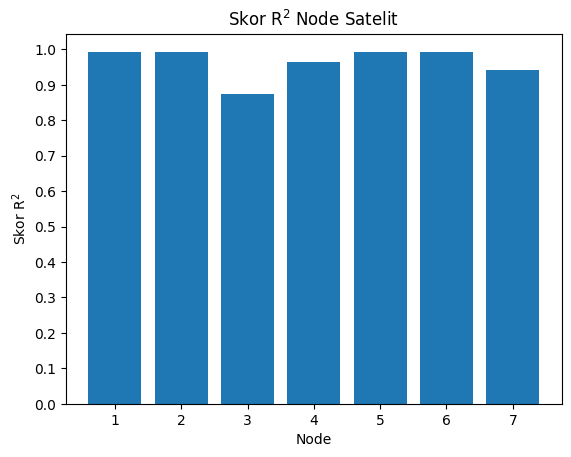
\includegraphics[width=0.6\textwidth]{fig/r2_2018-05-19.png}
\caption{Plot Skor R2 Model 19 Mei 2018}
\label{fig:r219}
\end{center}
\end{figure}

\begin{figure}[H]
\setlength\belowcaptionskip{-0.7\baselineskip}
\begin{center}
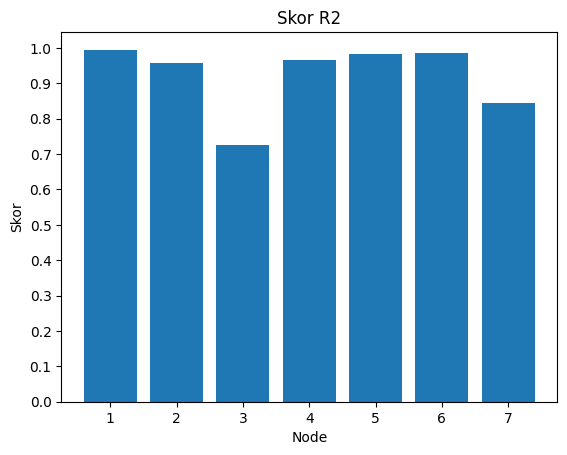
\includegraphics[width=0.6\textwidth]{fig/r2_2018-05-20.png}
\caption{Plot Skor R2 Model 20 Mei 2018}
\label{fig:r220}
\end{center}
\end{figure}

Selanjutnya, keakuratan model termal dalam memprediksi suhu \textit{node} satelit pada
periode observasi dapat dilihat dari nilai \textit{root mean square error} (RMSE)
model yang mengukur seberapa jauh nilai suhu hasil prediksi model dengan nilai
suhu hasil observasi data telemetri. Gambar \ref{fig:rmse19} dan
\ref{fig:rmse20} memuat plot RMSE model termal. 

\begin{figure}[H]
\setlength\belowcaptionskip{-0.7\baselineskip}
\begin{center}
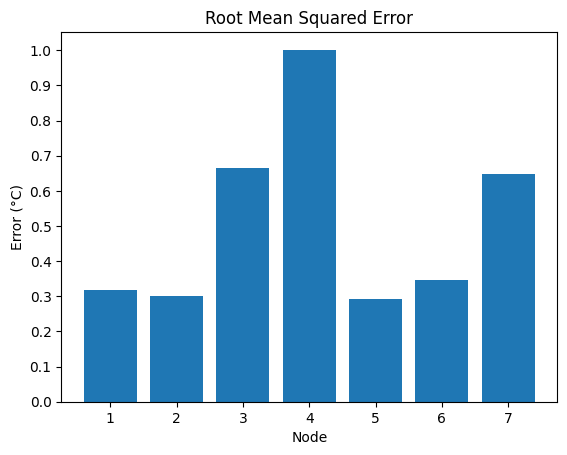
\includegraphics[width=0.6\textwidth]{fig/rmse_2018-05-19.png}
\caption{Plot Nilai RMSE Model 19 Mei 2018}
\label{fig:rmse19}
\end{center}
\end{figure}

\begin{figure}[H]
\setlength\belowcaptionskip{-0.7\baselineskip}
\begin{center}
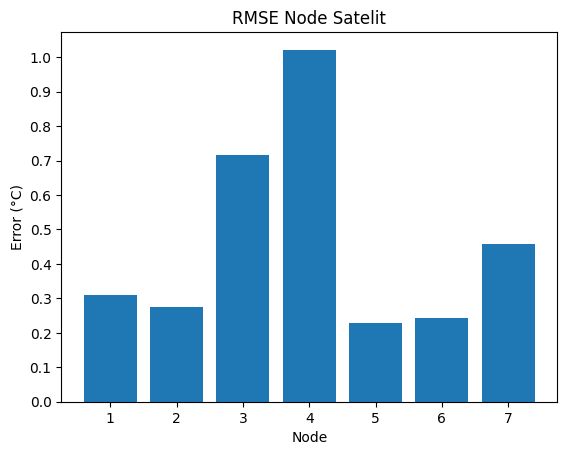
\includegraphics[width=0.6\textwidth]{fig/rmse_2018-05-20.png}
\caption{Plot Nilai RMSE Model 20 Mei 2018}
\label{fig:rmse20}
\end{center}
\end{figure}

Dapat dilihat bahwa plot RMSE model termal menunjukkan hasil yang agak berbeda
dari plot skor R2 model termal pada Gambar \ref{fig:r219} dan \ref{fig:r220}
sebelumnya. Nilai RMSE paling besar untuk kedua periode observasi sama-sama
diperoleh dari \textit{node} 4 disusul oleh \textit{node} 3 dan kemudian \textit{node} 7. \textit{Node} 4 konsisten
memiliki nilai RMSE lebih besar sedikit dari 1 \degree C untuk kedua periode
observasi. \textit{Node} 3 juga konsisten memiliki nilai RMSE lebih besar dari 0.6
\degree C untuk kedua periode observasi sedangkan \textit{node} 7 sempat menyentuh nilai
di bawah 0.5 \degree C pada periode observasi 20 Mei 2018.

Perlu diperhatikan bahwa nilai RMSE bergantung pada skala dan dataset yang
digunakan serta baru dihitung untuk iterasi pertama model termal. Karena itu,
perbedaan nilai maksimum dan minimum RMSE baru dapat disimpulkan setelah ada
perbandingan dengan model termal di masa depan. Dengan kata lain, belum dapat
disimpulkan apakah nilai error prediksi \textit{node} 4 model termal saat
ini adalah dapat dikategorikan rendah atau tinggi.

\section{Analisis}

Hasil pemodelan termal satelit LAPAN-A3 dari bagian sebelumnya menunjukkan
bahwa model termal yang dikembangkan sudah dapat memodelkan karakteristik
termal satelit LAPAN-A3 secara umum. Akan tetapi, akurasi model termal satelit
dalam memodelkan karakteristik termal \textit{node} 3, 4, dan 7 dapat dikatakan lebih
rendah dibandingkan dengan 4 \textit{node} lainnya dan masih perlu ditingkatkan. Node 3
dan 7 konsisten memiliki skor R2 lebih rendah dibandingkan \textit{node}-\textit{node} lainnya
sedangkan \textit{node} 4 memiliki nilai RMSE paling besar untuk kedua periode
observasi.

Dalam menganalisis hasil pemodelan termal, perlu diingat bahwa metrik
performa model yang dihitung hanya berlaku untuk iterasi model saat ini. Secara
spesifik, parameter RMSE bergantung pada skala pemodelan dan dataset yang
digunakan. Karena itu, perbedaan nilai maksimum dan minimum RMSE baru dapat
disimpulkan setelah ada perbandingan dengan model termal di masa depan. Dengan
kata lain, belum dapat disimpulkan apakah nilai RMSE \textit{node}-\textit{node} model termal
saat ini adalah dapat dikategorikan rendah atau tinggi.

Terlepas dari ketidakpastian dan ketidakakuratan bawaan dari metode numerik dan Machine
Learning yang digunakan pada karya tulis ini, dapat diduga bahwa model satelit LAPAN-A3 yang
digunakan belum dapat mewakili seluruh karakteristik termal satelit. Dengan
menganalisis sumber ketidakakuratan model yang potensial, model termal satelit
dapat dikembangkan lebih lanjut pada iterasi berikutnya. Harapannya, iterasi
model termal satelit berikutnya dapat menunjukkan performa yang jauh lebih
akurat lagi.

Pertama, satelit LAPAN-A3 didekati dengan model 7 \textit{node} diskrit yang
mewakili 6 sisi satelit serta 1 plat tengah satelit. \textit{Node} digunakan sebagai
satuan titik analisis terkecil sehingga bagian satelit yang diwakili \textit{node}
dianggap memiliki suhu yang sama. Parameter kapasitas termal yang digunakan
pada persamaan-persamaan termal di karya tulis ini pun adalah nilai kapasitas
termal rata-rata \textit{node}. 

\textit{Node} satelit yang terdiri dari material dan komponen yang berbeda dapat
menghasilkan rentang kapasitas termal \textit{node} yang besar juga. Rentang kapasitas
termal yang besar berarti rentang perubahan suhu antar material dalam \textit{node} yang
besar juga. Akibatnya, bacaan sensor suhu bisa saja berbeda jauh dengan suhu
komponen masing-masing sebenarnya.

Dalam konteks LAPAN-A3, \textit{node} 3 terletak di sumbu Y+ satelit yang memuat adaptor
roket dan \textit{separation ring} sedangkan \textit{node} 7 terletak di plat tengah
satelit yang menyimpan banyak komponen seperti komputer satelit dan sub-sistem
lainnya. Dengan begitu, karakteristik termal material pada kedua \textit{node} mungkin
tidak dapat terwakili seluruhnya dalam model satelit 7 \textit{node}. Agar karakteristik
termal dapat dimodelkan lebih akurat, jumlah \textit{node} yang digunakan dalam
pemodelan dapat ditambah.

Kemudian, satelit LAPAN-A3 juga diasumsikan berbentuk balok sehingga
perhitungan \textit{view factor} dari \textit{node} ke Bumi disederhanakan menjadi plat
persegi panjang ke Bumi. Pada kenyataannya, satelit memiliki komponen yang
tidak berbentuk persegi panjang seperti antena dan kamera. Penambahan jumlah
\textit{node} untuk memastikan komponen-komponen tersebut terwakili tentunya juga akan
menambah akurasi dari model termal satelit. Selain itu, tidak tertutup juga
penggunaan metode elemen hingga untuk menghitung nilai \textit{view factor}
secara terpisah.

Lalu, dari Persamaan \ref{eq:lineq} dapat dilihat juga bahwa perubahan suhu
suatu \textit{node} dipengaruhi perubahan suhu \textit{node}-\textit{node} lainnya akibat adanya
perpindahan panas lewat konduksi dan radiasi antar \textit{node}. Karena itu, perlu
dilakukan analisis inferensi lebih lanjut untuk menentukan suku-suku dominan
dalam Persamaan \ref{eq:lineq} yang mungkin menyumbang error paling besar. Jika
hasil analisis lebih lanjut menunjukkan bahwa perubahan suhu \textit{node} 4 didominasi
oleh pengaruh perubahan suhu \textit{node} 3 dan 7, penjelasan sebelumnya dapat menjawab
hasil nilai RMSE \textit{node} 4. Sebaliknya, hasil analisis tersebut dapat digunakan
untuk melihat akurasi suku termal mana yang perlu ditingkatkan.

Analisis untuk melihat dampak tiap suku dalam Persamaan \ref{eq:lineq} tidak
dilakukan dalam karya tulis ini karena membutuhkan modifikasi persamaan termal
untuk turut memperhitungkan hubungan antar variabel independen. Dapat dilihat
dari persamaan tersebut bahwa variabel suhu \textit{node} berkorelasi erat dengan
variabel suhu \textit{node} pangkat 4. Jika salah satu variabel diketahui, variabel
lainnya dapat dihitung juga. 

Fenomena adanya korelasi tinggi antar variabel independen di atas dinamakan
kolinearitas. Meski tidak berdampak banyak pada akurasi prediksi model,
harus diperhitungkan dalam analisis untuk menghitung dampak suku termal pada
persamaan termal secara individual \cite{lieberman2014}\cite{mundfrom2018}.
Kolinearitas dapat diatasi dengan menyeleksi variabel independen sehingga tidak
ada kolinearitas pada variabel yang tersisa atau menggunakan metode pemodelan
regresi linear lain yang tidak terpengaruh kolinearitas.

